\chapter{How the Agent Works}\label{ch:agent}

\section*{Introduction}
\addcontentsline{toc}{section}{Introduction}

A capable model on its own does not solve the actual problem. Handed a
question like ``which regions have upsell opportunity for 5G,'' qwen3
cannot just answer. It does not know the schema, it cannot see the
database, and even if it could write one correct query, plenty of real
questions need more than one query chained together before there is
enough to answer from. So what actually turns a single model call into
something that can do that? The loop wrapped around it: read the
question, decide on an action, observe what came back, and either take
another action or conclude. And that loop is not new to this chapter ---
it is the exact same idea the first local prototype in Chapter~\ref{chapter:BF-DFP} was
already built around. What changed between then and now is not the
architecture, it is how reliably the model's chosen action gets
communicated back to the code running it. There is also a difference in
what the loop is running against: the previous chapter established that
the database underneath it never sits still, so everything the agent
does here --- every query, every chart, every exported row --- is read
against a target that is actively moving, not a fixed snapshot. This
chapter covers how that loop actually works today, how it grounds
itself in the real schema instead of guessing, how it catches its own
mistakes before they reach the user, and everything it can do beyond
just answering in text. And it is worth flagging what to watch for while reading
it. Chapter~\ref{ch:context}, Section~\ref{sec:challenges}, laid out three gaps
that started this whole project off: raw data that never quite becomes actionable
insight, churn scores that live somewhere the people who need them do not look,
and a wait between asking a business question and getting an answer backed by
real data. Everything from here on is those three being handled one at a time, so
it is worth keeping them in mind as each piece goes past.

\section{The Loop: One Consistent Idea, Two Implementations}

Strip away everything specific to Bedrock or tool-calling, and the
agent's architecture is the same simple cycle it has been since
Chapter~\ref{chapter:BF-DFP}: \emph{perceive, decide, act, observe, repeat} --- read the
question and whatever has been learned so far, decide on exactly one
action, take it, look at what came back, and either take another action
or conclude with a final answer. This is the same reason-act-observe
pattern behind the ReAct approach to language-model agents~\cite{react}:
interleaving reasoning steps with concrete actions against the outside
world, rather than asking the model to reason its way to an answer in
one shot. Figure~\ref{fig:agent-loop} shows this cycle as it runs today.

What actually changed between the local Ollama prototype and the
current agent is not this cycle, but how an ``action'' gets expressed
and recognized. In Chapter~\ref{chapter:BF-DFP}, the model wrote a plain-text tag ---
\texttt{QUERY\_SC:}, \texttt{QUERY\_OP:}, or \texttt{CONCLUDE:} ---
followed by whatever it wanted to run or say, and the code on this end
parsed it back out with regular expressions. It worked, however nothing 
forced the model to follow that format specifically, as it drifts slightly to 
the step failed, without any clean way for the loop to recover.

To solve that issue, Bedrock's tool calling replaced the convention with a schema: a
fixed set of tools, each having an input shape, validated by the API before the loop sees anything:

\begin{itemize}
    \item \texttt{run\_sql(database, query)} --- execute a SQL query
    against the network or commercial database and return the rows.
    \item \texttt{inspect\_schema(table)} --- look up the real columns
    of a table before writing a query against it, rather than guessing.
    \item \texttt{conclude(text, recommendations, chart, ...)} --- end
    the loop with a final answer, optionally attaching a chart,
    recommendations, or a visualization spec.
    \item \texttt{propose\_action(description)} --- instead of
    answering, propose an operational action (a campaign, an SMS, a
    network flag) for a human to review, rather than taking it directly.
\end{itemize}

The loop itself did not need to change to adopt this --- it still asks
``what is the next action,'' takes it, and observes the result. What
changed is that ``the next action'' is now a structured tool call
instead of a string that has to be hoped for and parsed, which is what
makes the whole system meaningfully more reliable than the Chapter~\ref{chapter:BF-DFP}
version, not a difference in the underlying idea.

\begin{figure}[H]
\centering
\definecolor{agentblue}{HTML}{4A6FA5}
\definecolor{toolgray}{HTML}{6B7280}
\definecolor{concgreen}{HTML}{2E8B57}
\definecolor{actamber}{HTML}{B5793A}
\resizebox{\textwidth}{!}{%
\begin{tikzpicture}[
  qbox/.style={rectangle, rounded corners=3pt, draw=black!60, thick,
    fill=black!4, align=center, text width=4.4cm, inner sep=8pt, font=\footnotesize},
  agentbox/.style={rectangle, rounded corners=4pt, draw=agentblue, very thick,
    fill=agentblue!10, align=center, text width=5.6cm, inner sep=10pt, font=\bfseries\footnotesize},
  toolbox/.style={rectangle, rounded corners=3pt, draw=toolgray, thick,
    fill=toolgray!8, align=center, text width=4.6cm, inner sep=7pt, font=\footnotesize\ttfamily},
  obsbox/.style={rectangle, rounded corners=3pt, draw=toolgray, thick,
    fill=toolgray!15, align=center, text width=6.2cm, inner sep=7pt, font=\footnotesize},
  concbox/.style={rectangle, rounded corners=3pt, draw=concgreen, thick,
    fill=concgreen!10, align=center, text width=4.6cm, inner sep=7pt, font=\footnotesize\ttfamily},
  ansbox/.style={rectangle, rounded corners=3pt, draw=concgreen, very thick,
    fill=concgreen!18, align=center, text width=4.6cm, inner sep=8pt, font=\bfseries\footnotesize},
  actbox/.style={rectangle, rounded corners=3pt, draw=actamber, thick,
    fill=actamber!12, align=center, text width=4.6cm, inner sep=7pt, font=\footnotesize\ttfamily},
  humbox/.style={rectangle, rounded corners=3pt, draw=actamber, very thick,
    fill=actamber!20, align=center, text width=4.6cm, inner sep=8pt, font=\bfseries\footnotesize},
  lbl/.style={font=\scriptsize\itshape, align=center},
]

\node[qbox] (q) {User Question\\[2pt]\normalfont\scriptsize (plus anything already learned this turn)};
\node[agentbox, below=9mm of q] (agent) {Agent\\[2pt]\normalfont\footnotesize reasons over the question and decides exactly one next action};

\node[toolbox, below=16mm of agent, xshift=-6.2cm] (runsql) {run\_sql(\allowbreak database,\allowbreak query)};
\node[toolbox, right=8mm of runsql] (inspect) {inspect\_schema(\allowbreak table)};
\node[obsbox, below=8mm of $(runsql.south)!0.5!(inspect.south)$] (observe) {Observe: query results, or the real columns of a table};

\node[concbox, below=16mm of agent, xshift=6.2cm] (conclude) {conclude(\allowbreak text,\allowbreak chart,\allowbreak ...)};
\node[actbox, right=8mm of conclude] (propose) {propose\_action(\allowbreak description)};
\node[ansbox, below=8mm of conclude] (answer) {Final Answer\\[2pt]\normalfont\footnotesize shown to the user};
\node[humbox, below=8mm of propose] (human) {Human Review\\[2pt]\normalfont\footnotesize (Ops Portal)};

% forward flow
\draw[-{Latex[length=2.5mm]}, thick] (q) -- (agent);
\draw[-{Latex[length=2.5mm]}, thick] (agent.south) -- ++(0,-4mm) -| (runsql.north);
\draw[-{Latex[length=2.5mm]}, thick] (agent.south) -- ++(0,-4mm) -| (inspect.north);
\draw[-{Latex[length=2.5mm]}, thick] (runsql.south) -- (observe.north -| runsql.south);
\draw[-{Latex[length=2.5mm]}, thick] (inspect.south) -- (observe.north -| inspect.south);
\draw[-{Latex[length=2.5mm]}, thick] (agent.south) -- ++(0,-4mm) -| (conclude.north);
\draw[-{Latex[length=2.5mm]}, thick] (agent.south) -- ++(0,-4mm) -| (propose.north);
\draw[-{Latex[length=2.5mm]}, thick] (conclude) -- (answer);
\draw[-{Latex[length=2.5mm]}, thick] (propose) -- (human);

% the loop-back — this is the actual cycle
\draw[-{Latex[length=2.5mm]}, thick, agentblue]
  (observe.west) to[out=180, in=270] node[lbl, agentblue, xshift=-2mm] {repeat until\\ready to conclude}
  ++(-2.6cm, 1.8cm) |- (agent.west);

\end{tikzpicture}%
}
\caption{The agent's reasoning loop. \texttt{run\_sql} and
\texttt{inspect\_schema} feed back into another round of reasoning;
\texttt{conclude} and \texttt{propose\_action} end it.}
\label{fig:agent-loop}
\end{figure}


\begin{figure}[H]
\centering
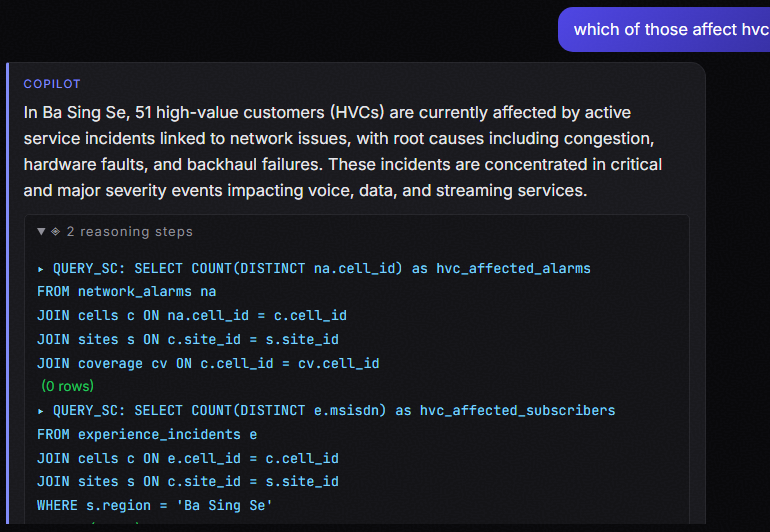
\includegraphics[width=0.8\textwidth]{figures/ch5-steps-panel-b.png}
\caption{The steps panel under a finished answer. The first \texttt{run\_sql}
returned no rows and is left visible rather than hidden.}
\label{fig:ch5-steps-panel}
\end{figure}

Figure~\ref{fig:agent-loop} is the theory. Figure~\ref{fig:ch5-steps-panel}
is what it actually looks like when the loop runs against a real
question --- every \texttt{run\_sql} step gets logged and shown to the
user, so the loop is not a black box even though the reasoning behind
each step is not shown in full.
\section{Knowing When Not to Answer Yet}

The first decision the loop makes is not which query to run. It is whether
the question can be answered honestly as asked.

Take a question the dashboard gets constantly: ``5G upsell opportunities
by region.'' That sounds specific enough. It is not. Does it mean every
subscriber holding a 5G-capable handset who is still on a 4G plan? Only
the high-value ones, because a campaign budget is finite? Only the ones
who are also showing churn risk, because those are the ones worth
spending a retention offer on? Those are three different lists, three
different campaigns, and three different costs. An agent that quietly
picks one and answers looks confident and is probably answering a
question nobody asked --- and, worse, the answer gives no clue which
reading it used.

So before running anything, the agent checks whether it should ask first.
Three gates, cheapest first, and most questions pass straight through all
three without paying for any of them:

\begin{table}[H]
\centering
\small
\begin{tabular}{@{}p{2.9cm}p{4.5cm}p{5.0cm}@{}}
\toprule
\textbf{Trigger} & \textbf{Looks like} & \textbf{What the agent does} \\
\midrule
Threshold only a human can set
& ``high ARPU'', ``heavy data users'', ``above average''
& Asks for a number, with a ``pick a sensible one for me'' fallback \\
\addlinespace
Breakdown with no dimension
& ``show me a drilldown of subscribers''
& Offers the real drill paths --- region, technology, value segment \\
\addlinespace
Genuine vagueness
& ``what should we focus on'', ``biggest problems''
& Asks the model what is actually being requested \\
\bottomrule
\end{tabular}
\caption{The three cases where the agent asks before it queries.}
\label{tab:clarify-gates}
\end{table}


% =====================================================================
% SCREENSHOT NEEDED --- figures/ch5-clarify.png
% Where: chat UI (localhost:8000), Copilot tab.
% What to capture: ask "5G upsell opportunities by region" and capture the
% clarify card BEFORE clicking an option --- the question the agent asks
% plus the list of option buttons, ideally with the answer that follows
% after picking one visible underneath.
% =====================================================================
\begin{figure}[H]
\centering
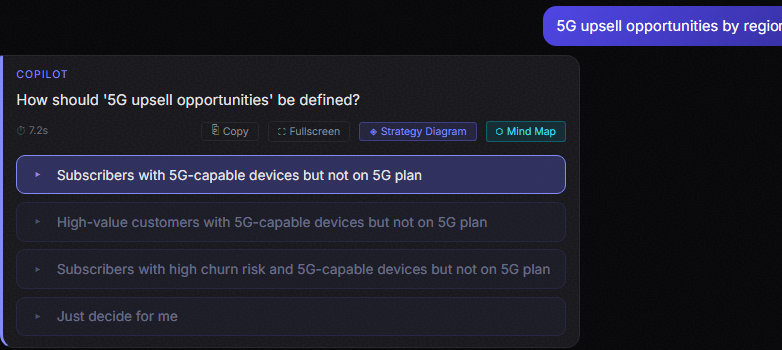
\includegraphics[width=0.85\textwidth]{figures/ch5-clarify1.png}
\caption{The agent declining to guess: three readings offered for ``5G upsell
opportunities by region'' before any query runs.}
\label{fig:ch5-clarify-ask}
\end{figure}

\begin{figure}[H]
\centering
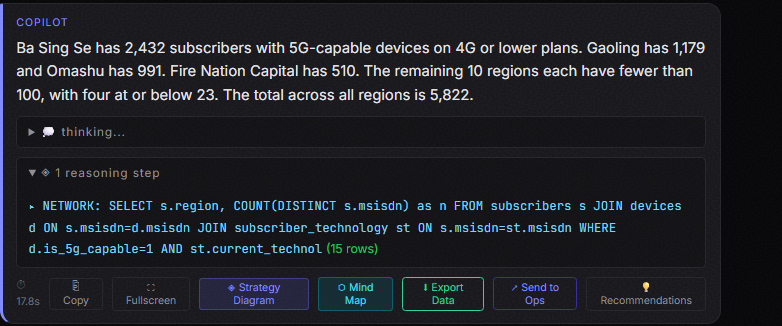
\includegraphics[width=0.85\textwidth]{figures/ch5-clarify2.png}
\caption{The answer, once a reading is chosen.}
\label{fig:ch5-clarify-answer}
\end{figure}


There are two details that make it behave like a tool/agent rather than 
a chatbot answering simple questions.


The options are \emph{complete standalone questions}, not dialogue turns.
Clicking ``High-value customers with 5G-capable devices but not on 5G
plan'' runs exactly that, as though it had been typed. There is no
half-remembered state waiting to be resumed, and nothing to go stale if
the user wanders off and asks something else instead. It also removes an
obvious way to build an infinite loop: the agent remembers which options
it just offered, so a clicked option runs directly instead of tripping
the same gate again and being asked to clarify its own clarification.

And the agent never asks the user to define a term the data already
defines. ``High-value customer'' is not a matter of opinion here --- it
is a column. Neither is ``having an issue right now,'' which is a row in
the live incident log with a timestamp on it. Questions like ``do we have
any HVCs with streaming issues right now'' therefore skip the whole gate
and run immediately, because every term in them is already pinned down by
the schema. Asking about those would not be careful, it would be
annoying.

The pattern here is the same one that runs through the rest of this
chapter. An agent that guesses and sounds certain is worse than one that
admits the question has more than one reading, in exactly the way an
answer built on numbers it never queried is worse than one that says it
does not know.

\section{Grounding the Agent in Domain Knowledge}

Knowing the four tools is one thing. Knowing which columns actually
exist in a twenty-plus table schema, or which of the two databases a
given question even belongs to, is another. So where does that
knowledge come from, if not from the model just knowing it?

Two different mechanisms, doing two different jobs, kept deliberately
separate. The first is a set of fixed behavioral rules baked directly
into the system prompt --- for example, a ranking principle that tells
the agent to compute every metric in one grouped query and never rank
by one number while quoting another. These are general, apply to every
question, and exist to fix \emph{reasoning} mistakes.

The second is retrieval: the same retrieval-augmented generation idea
behind giving a language model access to an external knowledge source
instead of relying purely on what it already knows~\cite{rag}, applied
here to schema and SQL knowledge rather than open-domain text. A schema
knowledge graph only injects the subgraph of tables and join paths
relevant to the current question, an intent classifier routes a
question toward the network side, the commercial side, or both, and a
hybrid search index --- BM25~\cite{bm25} keyword matching and FAISS-based
vector search~\cite{faiss}, merged --- surfaces telecom-specific SQL
patterns on demand. However this approach only half handles the knowledge gaps,
and it doesn't even work on the reasoning ones.

One might ask why should they be seperate when we can just cram 
everything into one long prompt? It's because a knowledge gap and a 
reasoning gap need different fixes, and mixing them up will lead 
to a whack-a-mole situation: you patch one bad query with a 
hardcoded example, and a slightly different question breaks it 
the same way. Having a general principle would generalize, but a one-off
example doesn't. 


A third, smaller mechanism sits between those two, and it exists because of a
failure neither of them caught. Asked to recommend a retention offer, the agent
would name a real product from the catalogue --- the names are in the schema, so
it had those --- then simply invent the terms attached to it. It proposed a
20\% discount on an offer the catalogue records at 15\%, and 30~GB of bonus data
on one that carries 50. Plausible, internally consistent, and wrong.

This is neither a reasoning gap nor a retrieval gap. Retrieval surfaces schema
--- table names, columns, join paths --- and the terms are row values, which it
never looks at. The catalogue is ten rows, so the fix was to stop retrieving
anything and put the whole thing in the system prompt.




The general form of that fix is worth stating, because it recurs: when a small
reference table governs what the agent is allowed to claim, putting the table in
context is cheaper and more reliable than either instructing the model to look
it up or checking its output afterwards. Terms are emitted structurally rather
than copied from the catalogue's free-text descriptions, which still quote a
currency the project has since moved away from --- a reminder that injected
context inherits whatever inconsistencies the source data carries.

\section{Catching the Model's Mistakes}

Grounding the agent in the right knowledge cuts down on mistakes. It
does not eliminate them, so the loop also has to catch what slips
through, on both ends: before a query runs, and before an answer
reaches the user.

Before a query runs, every SQL statement is checked against the real schema. If
it references a column that does not exist --- something models do often when a
table has many similarly-named fields --- the check fails before anything
executes, and the real column names are fed back so the model can correct itself
rather than guess again.

After a query runs, a second check reads the answer itself. Does every number it
cites appear in the rows just queried? Does any negative claim --- ``there are
no active alarms'' --- rest on a query that actually looked? If more than half
the significant numbers cannot be traced, or a negative claim was never checked,
the answer is regenerated once, restricted to what the results contain.

The system prompt already told the model to claim only what it had queried. It
still didn't. The difference is that a prompt asks and this check does not.
 Verified against the exact leaked output
that triggered this fix, plus a handful of regression cases to make
sure well-formed answers were left untouched.


\subsection{Claims About What Is \emph{Not} Happening}

Checking numbers catches made-up figures. It does absolutely nothing about a
different and frankly more dangerous kind of claim: saying that something is
not there.

The failure that led to this was very specific. Asked to explain a critical
power failure at a site, the agent gave a genuinely good answer --- right root
cause, right severity, right subscriber count, right timestamp --- and then went
ahead and added that the fault was localised and no other regions or
technologies were impacted. At that exact moment seven sites across six regions
had active incidents, one of them hitting six times as many subscribers as the
site being discussed. Nobody had even asked about other regions. The agent just
volunteered a negative it had never once queried.

A wrong number is embarrassing. A confident ``nothing else is affected'' sends
an operator to the wrong fault, which is worse.

The system prompt already had an explicit rule in it --- claim only what you
queried --- and the model went straight past it. That is the lesson this chapter
keeps running into: telling the model something is a request, and a request is
not a guarantee. So the rule gets enforced afterwards instead. Answers are scanned for
scope-and-exclusivity negatives (\emph{no other}, \emph{nothing else},
\emph{isolated to}, \emph{not a network-wide}, \emph{no active alarms},
\emph{no evidence of}, \emph{not linked to}), and when one is found the check
asks a single question: did any query in this turn actually look and come back
empty?

That question has a precise answer sitting right there. A query that returns
zero rows gets recorded as such in the step log, and contributes nothing to the
result text, because there are no rows to contribute. Which makes its presence
exactly the evidence a negative claim needs. A negative with a zero-row query
behind it is earned and passes straight through. A negative with nothing behind
it triggers the same regeneration path as a made-up number, with an extra
instruction to delete the claim rather than soften it.

I validated the check in both directions: against the four real failures seen
during this project, all of which it catches, and against ordinary answers full
of counts and comparisons, none of which it touches. The line it draws is not
between confident and hedged language. It is between a claim that has a query
behind it and a claim that does not.

\section{Beyond Answering: Actions and Visuals}

Not every question is best answered with a paragraph. The
\texttt{conclude} tool can attach a chart, a drill-down mind map, or a
two-column strategy diagram alongside the text, letting the agent
choose a visual when a visual is actually the right answer --- a
regional breakdown is a bar chart, not three sentences trying to
describe one.

% =====================================================================
% SCREENSHOT NEEDED --- figures/ch5-chart-example.png
% Where: chat UI, Copilot tab.
% What to capture: any question that naturally produces a Plotly chart
% in the answer (bar/pie/treemap --- e.g. "technology distribution by
% region" or "ARPU by segment"). Capture the rendered chart itself,
% ideally with its title/legend visible.
% =====================================================================
\begin{figure}[H]
\centering
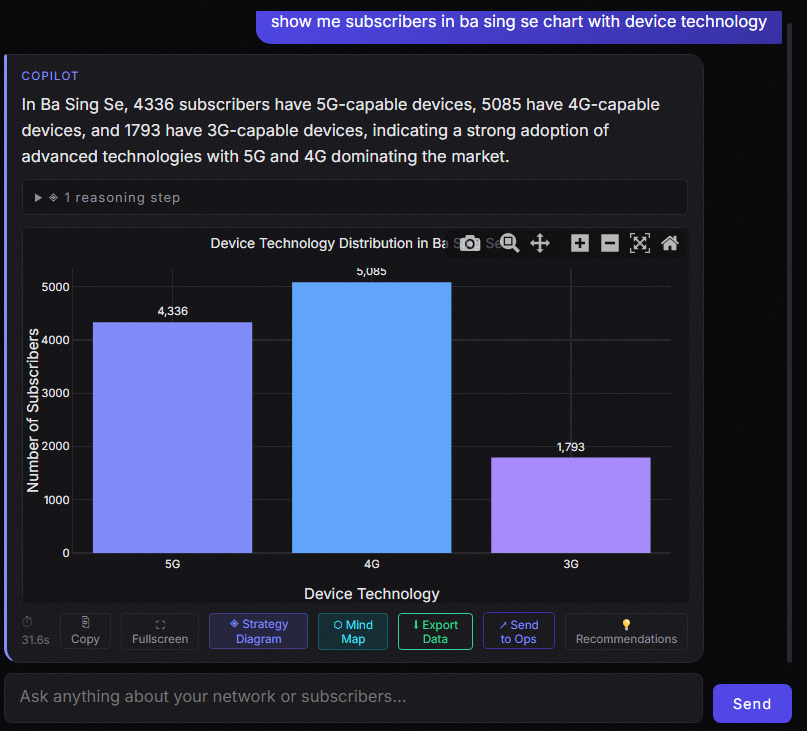
\includegraphics[width=0.85\textwidth]{figures/ch5-chart-example.png}
\caption{A Plotly chart attached to a \texttt{conclude} call, built directly
from the query results.}
\label{fig:ch5-chart}
\end{figure}

For anything that is really a hierarchy rather than a flat comparison
--- subscribers broken down by region, then technology, then value
segment --- the mind map is the better fit: an interactive drill-down
tree the user can expand, collapse, or re-root into a single branch,
rather than a static image.

% =====================================================================
% SCREENSHOT NEEDED --- figures/ch5-mindmap-example.png
% Where: chat UI, Copilot tab. Click the "Mind Map" button under an
% eligible answer, or ask a drilldown question directly (e.g.
% "drilldown of subscriber counts by region, technology, and value
% segment"). Capture the mind map expanded a couple of levels deep,
% ideally showing the toolbar (layout cycle / expand / collapse / fit).
% =====================================================================
\begin{figure}[H]
\centering
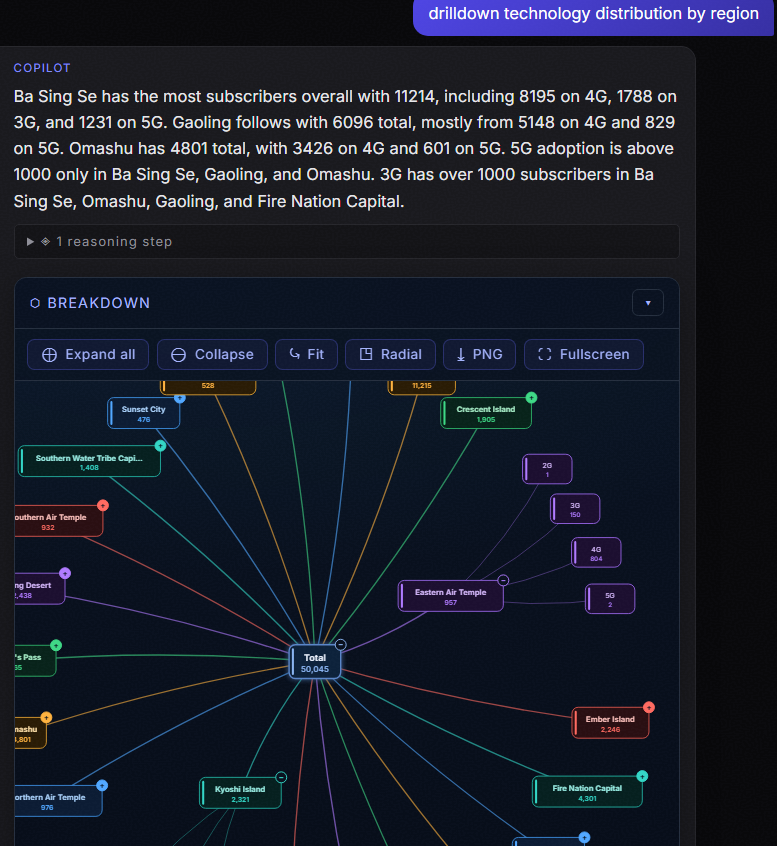
\includegraphics[width=0.85\textwidth]{figures/ch5-mindmap-example.png}
\caption{The drill-down mind map, one region expanded. Every node opens on
click --- this is one frame of something the user drives.}
\label{fig:ch5-mindmap}
\end{figure}

The strategy diagram goes one step further than visualizing the data:
it pairs each subscriber segment with a recommended commercial
strategy, laid out as two connected columns so the segment-to-strategy
mapping is visible at a glance rather than buried in a paragraph.

% =====================================================================
% SCREENSHOT NEEDED --- figures/ch5-strategy-diagram.png
% Where: chat UI, Copilot tab. Click the "Strategy Diagram" button under
% an eligible answer (commercial/upsell/churn-flavored questions).
% What to capture: the two-column diagram with segments on one side,
% strategies on the other, and the connecting lines between them.
% =====================================================================
\begin{figure}[htbp]
\centering
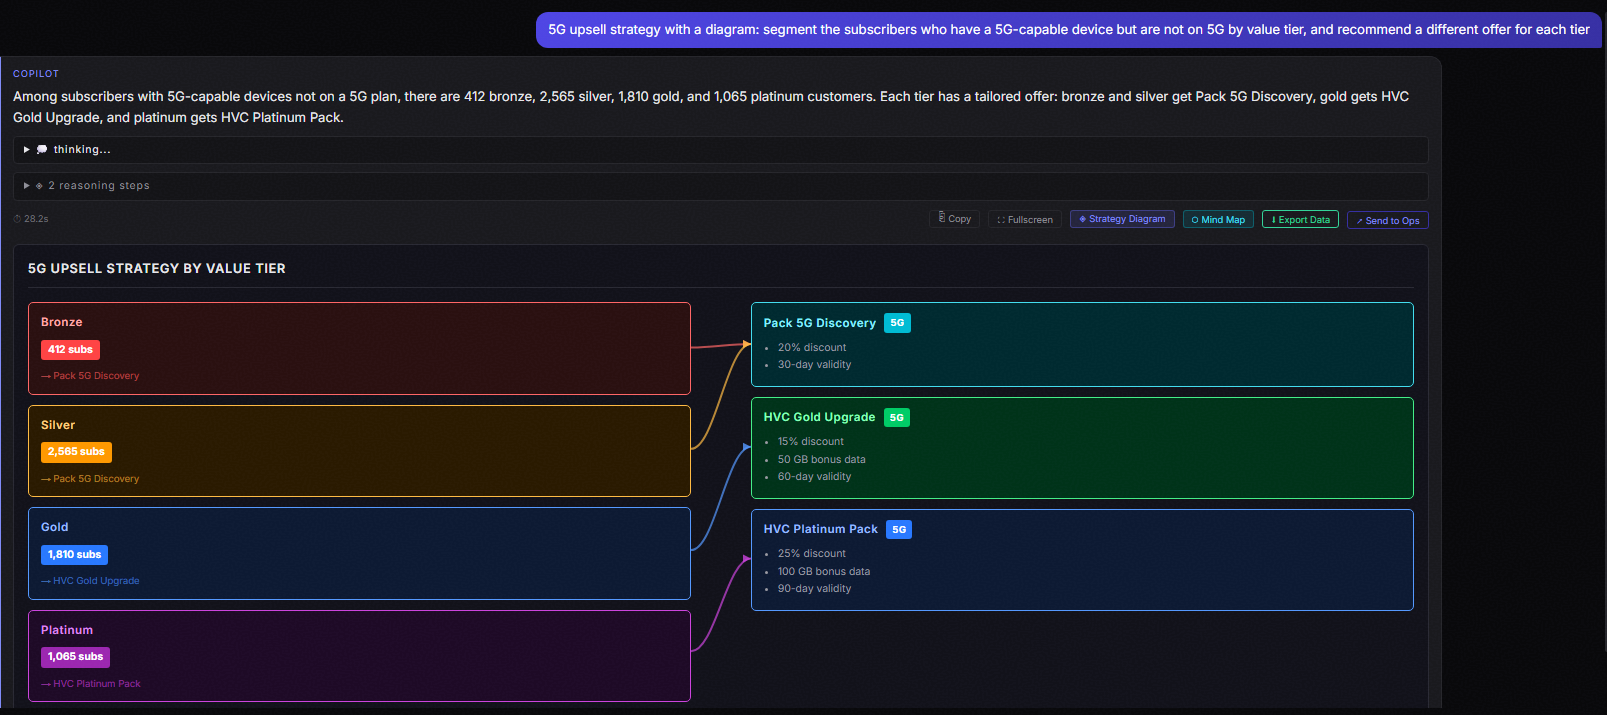
\includegraphics[width=0.85\textwidth]{figures/ch5-strategy-diagram.png}
\caption{The strategy diagram, mapping subscriber segments to
recommended commercial actions.}
\label{fig:ch5-strategy}
\end{figure}

The last of the ``beyond text'' outputs is the export button: any
answer built from row-level data (subscribers, devices, cells) can be
exported as a CSV, and the export query is not just the original
query re-run --- the model is asked to add one to three annotation
columns (\texttt{recommended\_action}, \texttt{priority},
\texttt{campaign\_type}) computed with SQL \texttt{CASE WHEN} logic, so
the export is directly actionable rather than a raw data dump someone
still has to interpret.

% =====================================================================
% SCREENSHOT NEEDED --- figures/ch5-csv-export.png
% What to capture: the exported CSV from a subscriber-level answer,
% opened in Excel/LibreOffice, with the extra annotation columns
% (recommended_action / priority / campaign_type) visible alongside the
% real data columns.
% =====================================================================
\begin{figure}[htbp]
\centering
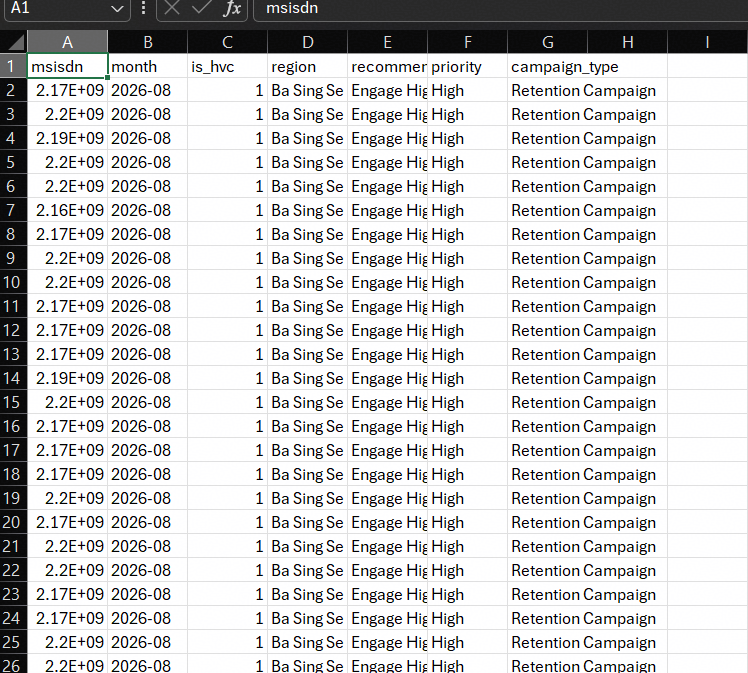
\includegraphics[width=0.85\textwidth]{figures/ch5-csv-export.png}
\caption{An exported CSV with LLM-annotated columns added on top of the
raw query results.}
\label{fig:ch5-csv}
\end{figure}

\subsection{Proposing Actions: the Agent Does Not Get to Act Alone}

The \texttt{propose\_action} tool works on a different principle
entirely from the three above: the agent does not get to act on its
own. This is the one tool that reaches outside the chat portal, and it
is deliberately built so that reaching outside never means acting
outside without a human in the loop.

When the agent calls \texttt{propose\_action}, the chat server does not
touch the database at all. It publishes the proposal --- a campaign, an
SMS, a network flag --- to an MQTT~\cite{mqtt} topic, which is picked up by a
second, entirely separate server: the ops portal. That portal writes
the proposal into an \texttt{agent\_actions} table as \emph{pending}
and surfaces it in a human review queue. Only once a human approves it
(optionally editing the SMS text or the target audience first) does
anything actually get written to the commercial database --- a real
campaign row, a real SMS log entry. Deny it, and nothing happens at
all. The agent itself never executes anything; it only ever proposes.

% =====================================================================
% SCREENSHOT NEEDED --- figures/ch5-ops-review.png
% Where: ops portal (localhost:8001). What to capture: the review queue
% showing a pending action proposed by the agent (a campaign or SMS),
% ideally with the review modal open showing the Approve/Deny buttons.
% =====================================================================
\begin{figure}[htbp]
\centering
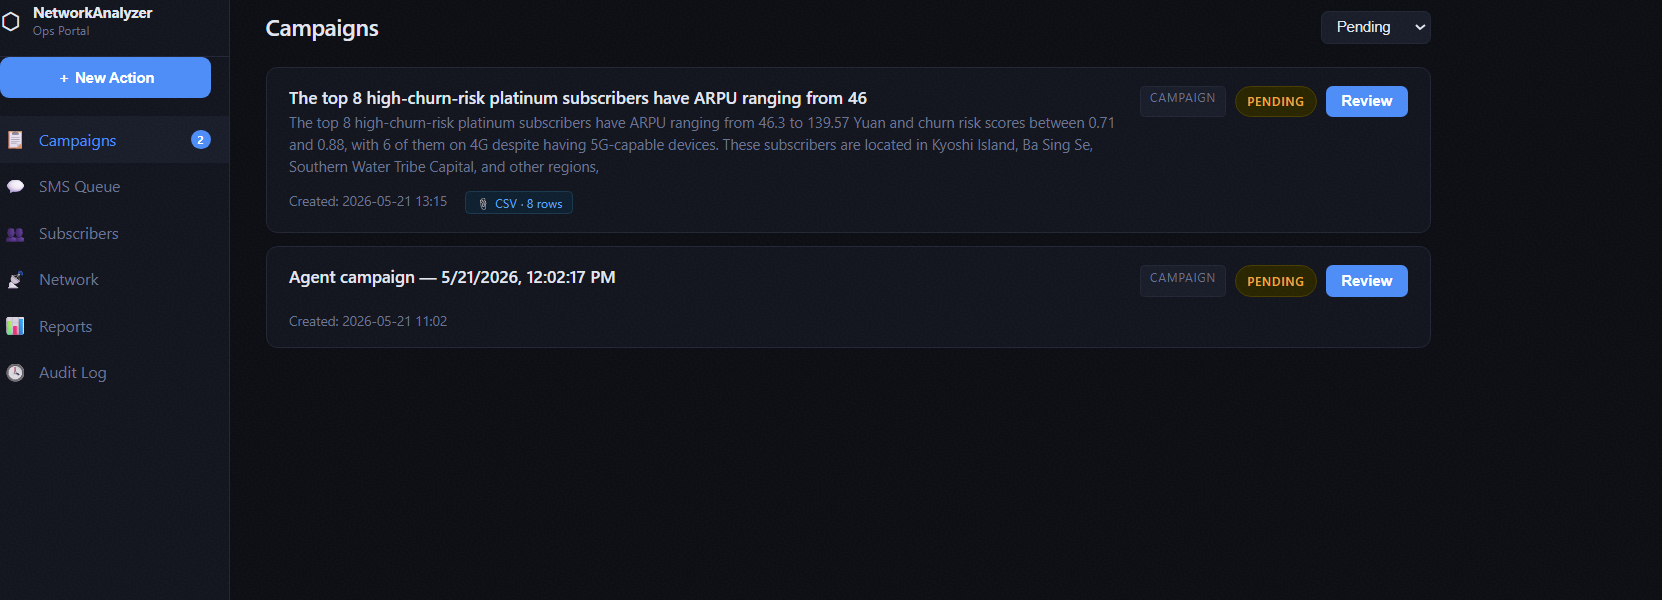
\includegraphics[width=0.85\textwidth]{figures/ch5-ops-review.png}
\caption{A proposed action waiting for human review in the ops portal,
having arrived there over MQTT from the chat server.}
\label{fig:ch5-ops-review}
\end{figure}



\section{Staying Fast: the Fast Path and the Semantic Cache}

The full loop in Figure~\ref{fig:agent-loop} is built for questions
that genuinely need multiple steps of reasoning. Running the entire
loop for something like ``how many 5G subscribers are there'' would
work, but it is a lot of machinery for a question with a one-query
answer, and it is slow for no reason.

Two shortcuts sit in front of the loop to avoid that waste. The first
is a fast path: questions recognized as a single simple metric skip
the loop entirely and go straight to a single-shot query, cutting the
usual multi-step latency down to one call. The second is a semantic
cache: if a new question is close enough (cosine similarity of at
least 0.92 against a recent question's embedding) to something already
answered this session, the cached result comes back immediately
instead of re-running the loop. That threshold is set deliberately
high --- a looser one would start returning the answer for ``drop rate
in the Fire Nation'' to a question about the Water Tribe, which is
worse than just being slow.

\section{Remembering the Conversation}

None of this works turn to turn without some notion of memory, since
the model itself is stateless --- every call starts from nothing
unless the conversation so far is fed back in explicitly. The
straightforward option, replaying every prior turn verbatim on every
new question, gets expensive fast in a long conversation. The other
extreme, summarizing everything, loses the specific numbers and
phrasing a follow-up question often depends on.

The agent splits the difference: the most recent turns are kept and
replayed verbatim, so a direct follow-up (``what about last month
instead'') has the exact prior context to work from, while anything
older than that gets folded into a running summary instead of being
dropped outright. The conversation the model actually sees on any
given turn is therefore a mix of a short gist of the early part of the
conversation plus the real, unedited recent turns --- bounded cost,
without hard-forgetting anything that happened earlier in the session.
It is similar in spirit to how long-running AI assistants keep a
conversation going well past what would otherwise fit in a single
context window --- recent turns kept exact, older ones compressed into
a summary rather than dropped --- just applied here at a far smaller
scale, over a handful of turns instead of an entire extended session.

\section*{Conclusion}
\addcontentsline{toc}{section}{Conclusion}

This chapter walked through what actually turns a single Bedrock call
into an agent: the same perceive-decide-act-observe loop the very
first local prototype used, now expressed through structured tool
calls instead of hoped-for text tags. Grounding keeps that loop
pointed at the real schema instead of guessing, mistake-catching
stops bad SQL and ungrounded answers before they reach the user, and
the conclude/propose\_action split gives the agent a way to act beyond
plain text --- charts, mind maps, strategy diagrams, CSV exports, and
proposals that only ever become real through a human in the ops
portal --- without ever acting unsupervised. And because the database
underneath all of it never holds still, as Chapter~\ref{ch:livingdb} established, the
fast path, the cache, and the memory system all exist for the same
reason: to keep a system reasoning over a moving target fast,
consistent, and honest. Between what Chapter~\ref{ch:livingdb} and this chapter
covered, the core of the project is now on the table --- a live,
self-updating environment, and an agent that can actually reason over
it without acting alone.
